% \section{Introduction}
% 
% The proposed D.Phil will be a continuation of my previous work on designing and commissioning parts of the South African C-BASS antenna. In the immediate future we are planning to build a Field Programmable Gate Array (FPGA) based digital receiver, to replace the existing analogue system (see %\fign{fig:analog_receiver}) designed by Dr. Oliver King as part of his D.Phil. Thesis \cite{oliver_2009}. The design of this new digital receiver is under way using a development environment made possible by the University of California (Berkeley) Collaboration for Astronomy Signal Processing and Electronics Research (CASPER) group. This document can not begin to elucidate the details of the work, however every effort has been made to convey, broadly, the nature of the work to be undertaken.

\section{Introduction}



The C-Band All Sky Survey (C-BASS) has a goal of mapping the Galactic foreground in both polarisation and intensity in a 1~GHz band centred at 5~GHz.  The resolution of the survey will be approximately 0.8\degt, with a  rms noise level of \textless 100 $\mu$K per pixel. The large 1~GHz bandwidth was chosen to allow us to achieve high sensitivity across the entire sky in less than a year, while the 0.8\degt resolution is useful for Cosmic Microwave Background (CMB) experiments hoping to detect the predicted B-mode peak feature at a l$\approx$90 \cite{mortonson_2007}.  A detailed discussion of the CMB polarisation can be found in the literature (for example \cite{2002ApJ...578...12C}).  The experiment consists of two antennas located in the Owen's Valley Observatory (OVRO) in California (\fign{fig:ovroTelescope}) (deployed January 2009), and the MeerKAT support base in South Africa (\fign{fig:SaTelescope})  (deployed June 2009). My role in the project covers the development, deployment and commissioning of the Southern Hemisphere antenna (new digital receiver, control system commissioning, antenna surface measurements), as well as work on the analysis of Northern Hemisphere data obtained to date.


\begin{figure}
 \centering
 \subfloat[The completed OVRO antenna. The foam support of the secondary reflector which reduces scattering of incoming radiation compared to quadrupod support legs  and the metallic baffles installed around the primary reduce the far-out sidelobes.]{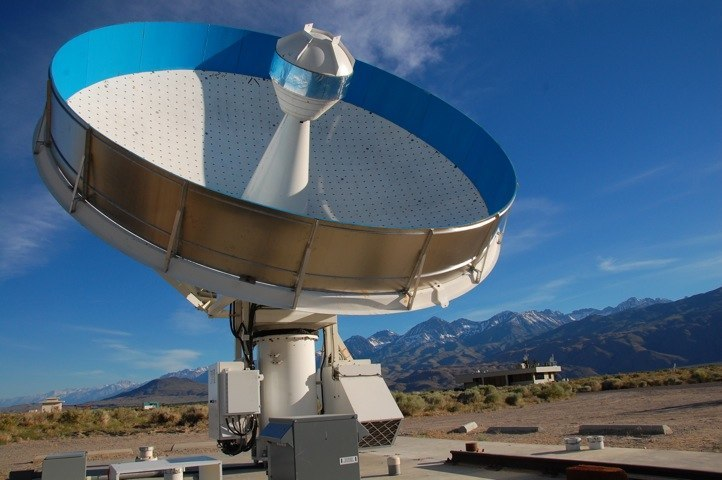
\includegraphics[height=0.4\textheight]{./images/antenna_photos/telescope.jpg}\label{fig:ovroTelescope}}\\
 \subfloat[The South African antenna installed at the Karoo site]{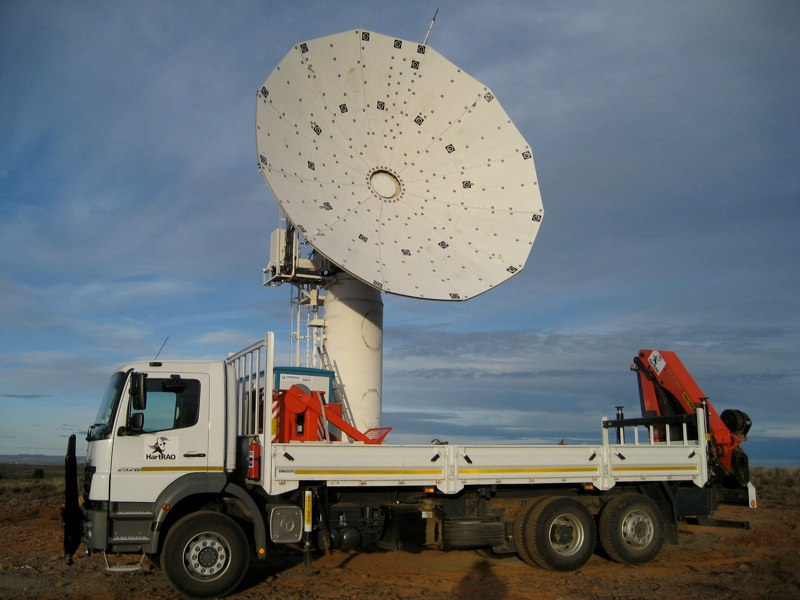
\includegraphics[height=0.4\textheight]{./images/antenna_photos/SAdish_installed_at_Karoo.jpg} \label{fig:SaTelescope}}
  \caption{Photographs of the Northern and Southern C-BASS antennas}
% OvroRays.jpg: 711x382 pixel, 72dpi, 25.08x13.48 cm, bb=
 %\caption{Ray Tracing of the OVRO antenna optical design. Notice the Gregorian optical layout}
 %\label{fig:ovroRays}
\end{figure}
